\documentclass{article}   

\usepackage{geometry}
\usepackage{qtree}
\usepackage[square,numbers]{natbib}
% \usepackage{cite}  
\geometry{a4paper}

\usepackage[]{algorithm2e}
\usepackage{amsthm}
\newtheorem{theorem}{Theorem}[section]
\newtheorem{corollary}{Corollary}[theorem]
\newtheorem{lemma}[theorem]{Lemma}

\usepackage[utf8]{inputenc}
\usepackage[T1]{fontenc}    % use 8-bit T1 fonts
\usepackage{lmodern}
\usepackage{hyperref}       % hyperlinks
\usepackage{lipsum}

\usepackage{color, colortbl}

\definecolor{Gray}{gray}{0.9}

\usepackage[protrusion=true,expansion=true]{microtype}

\usepackage{amssymb}
\usepackage{amsfonts}
\usepackage{eqnarray,amsmath}
\usepackage[table]{xcolor}

\usepackage{listings}
\usepackage{graphicx}
\usepackage{dirtytalk}

\usepackage{rotating}
\usepackage{caption}

%% if you use PostScript figures in your article
%% use the graphics package for simple commands
\usepackage{graphics}


%% or use the graphicx package for more complicated commands
\usepackage{graphicx}
\usepackage[table]{xcolor}

\usepackage{indentfirst}
\usepackage[utf8]{inputenc}
 \usepackage{subcaption}
\usepackage{xcolor}
 
\usepackage{xspace,color}
\usepackage{url}



\lstset{commentstyle=\color{red},keywordstyle=\color{black},
showstringspaces=false}
\lstnewenvironment{rc}[1][]{\lstset{language=R}}{}
\newcommand{\ri}[1]{\lstinline{#1}}  %% Short for 'R inline'

\lstset{language=R}             % Set R to default language


%https://tex.stackexchange.com/questions/96825/nicely-formatted-where-statement-for-maths
 \newenvironment{where}{\noindent{}where\begin{itemize}}{\end{itemize}}
 \renewcommand*\descriptionlabel[1]{\hspace\leftmargin$#1$}
 
\lstset{escapeinside={<@}{@>}}
% please place your own definitions here and don't use \def but
% \newcommand{}{}
%
% Insert the name of "your journal" with
% \journalname{myjournal}
%
\begin{document}

\title{%
  Practice 6: Statistical Tests} %\\~\\
  %\Large }
\author{Mayra Cristina Berrones Reyes 6291}

\maketitle

\section{Activity}

Please answer the next questions, taking into consideration the shared links.\\

\textbf{a) Describe the relationship between hypothesis testing and statistical tests.}\\

To understand the relationship between these two concepts, first we describe them separately.\\

A statistical test gives us a mechanism to be able to make quantitative decisions about processes. The goal of this decisions is to determine if there is enough evidence to \say{reject} a conjecture or hypothesis about our process. In this case, the conjecture is called null hypothesis \cite{montgomery2009}. A null hypothesis proposes that no significant difference exists in a set of given observations \cite{tdsc}.\\

A classical use of the statistical tests occurs in process control studies. \\

Hypothesis testing is a way we can test if the results of an experiment really have meaningful results. This means that we test to see if the results we have are valid by checking out the odds that said results could have happened by chance \cite{sthowto}. \\

It is very common in statistics to estimate a parameter from sample data. For example, a sample of the mean of the data is then used as the point estimate of the population mean. An hypothesis test addresses the uncertainty of the sample estimate, and instead of providing an interval, it attempts to refute a specific claim about a population parameter based on the sample data we took for the experiment \cite{montgomery2009}.\\

A common format for hypothesis test is shown in Listing \ref{list1}.\\

\begin{itemize}\label{list1}
\item $H_0$: Null hypothesis.
\item $H_a$: Alternative hypothesis.
\item Statistic test: This is based on the specific hypothesis test. 
\item Significance level: Commonly known as $\alpha$, defines the sensitivity of the test.
\item Critical value: This encompasses the values of the statistic test that lead to a rejection of the null hypothesis.
\end{itemize}

To answer the original question, seeing the common format for a hypothesis test, we can now say that they are both needed for a good analysis of the experimentation, because we should not just trust that the sample we took for our statistical analysis is the correct one, so we should combine engineering judgement with statistical analysis.\\
 
\textbf{b) What would indicate to reject the null hypothesis?}\\

To reject a null hypothesis we perform a statistical test, and then we compare its results with the critical value. If it is greater than the critical value, the hypothesis is rejected. A great explanation Jonathan Christensen \cite{stack1} says \say{In a theoretical underpinning, hypothesis tests are based on the notion of critical regions: the null hypothesis is rejected if the test statistic falls in the critical region. The critical values are the boundaries of the critical region. If the test is one sides, then there will only be one critical value, but in other cases there will be two.}\\

So we reject the null hypothesis if this falls in the critical value.\\

\textbf{c) How is the output of a statistical test interpreted?}\\

In this case, the output of the statistical test can be that we accept the null hypothesis, or we reject it. If ithe null hypothesis falls in the critical value, we reject it. The null hypothesis is a statement about belief \cite{montgomery2009}, so the test procedure is done in a way that the risk of rejecting the null hypothesis is small when it is in fact true. \\

\textbf{d) How to select the alpha value?}\\

The risk we mentioned in previous questions, $\alpha$, is often referred as value significance level of the test. When we use a small value of $\alpha$ it is often said that it actually proves something when the null hypothesis is rejected. \\

There is no magic significance level that will give us a 100\% accuracy results. The most common $\alpha$ values are $0.05$ and $0.01$, but they are mainly used based on tradition. Because this test are based in probability, there is always a chance of a wrong conclusion. \\

When doing this experiments, there are 2 types of errors, which are related and determined to the level of significance and the test used. So we should determine which error has worst concecuences for the experiment, before defining the risks.\\

In Table \ref{tab1} we name these type of errors.

\begin{table}[]\caption{Names and types of errors of the significance level.}\label{tab1}
\begin{tabular}{| p{3.2cm} | p{5cm} | p{5cm} | }
\hline
                         & \multicolumn{2}{ c |}{Truth about population}        \\              
\hline                                                                                                                                                 
Decision based on sample & $H_0$ is true                                                                                & $H_0$ is false    \\  
\hline                                                                                  
Fail to reject $H_0$     & Correct decision (Probability = $1-\alpha$)                                                  & \textbf{Type II error} Fail to reject $H_0$ when it is false (Probability = $\beta$) \\
\hline
Reject $H_0$             & \textbf{Type I error} Rejecting $H_0$ when is true (Probability = $\alpha$) & Correct decision (Probability = $1 - \beta$)    \\ 
\hline                                                    
\end{tabular}
\end{table}



\textbf{e) What are the most frequent misinterpretations of the \texttt{p}-value?}\\

The \texttt{p}-value is the probability of obtaining results at least as extreme as the observed results of a statistical hypothesis test, assuming that the null hypothesis is correct. It is the measure pf the probability that an observed difference may have occurred by random \cite{inv1}.\\

The incorrect interpretation of the \texttt{p}-value is very common. One of the most frequent is to interpret it as the probability of making a mistake by rejecting the true null hypothesis, which as we can see in Table \ref{tab1} is a Type I error.\\

Misinterpreting the \texttt{p}-value as the error rate creates the illusion that there is more evidence against the null hypothesis. But if we base the whole experiment on a study of \texttt{p}-value of 0.05, the difference observed in the sample may not exist in the whole population \cite{minitab}.\\

\textbf{f) What is the statistical power and what is it for?}\\

The statistical power of an experiment refers to how likely it is to distinguish an actual effect from one chance. It is the likelihood that the test we perform is correctly rejecting the null hypothesis, which looking at Table \ref{tab1} is the probability of avoiding Type II error \cite{stats1}. \\

A high statistical power means that the results we have are likely valid, and as the power increases, the probability of making a Type II error decreases.  It can be used as a tool to estimate the sample size required in order to detect an effect in an experiment \cite{sthowto2}.\\

\textbf{g) Examples of parametric and non-parametric statistical tests.}\\

The definition of non parametric is very convoluted, and better explained by examples. In Table \ref{tab2} we see examples of the type of analysis and the parametric and non parametric procedure.\\

\begin{table}[]\caption{Examples of different parametric and non parametric procedures for the same type of analysis.}\label{tab2}
\begin{tabular}{| p{6cm} | p{3.5cm} | p{3.5cm} | }
\hline
 \textbf{Analysis Type}&\textbf{Parametric} & \textbf{Non parametric}       \\              
\hline                                                                                                                                                 
Compare means between 2 distinct/independent groups& Two sample t-test&Wilcoxon rank sum test\\
\hline   
Compare 2 quantitative mesurements taken from the same individual&Paired t-test&Wilcoxon signed rank test\\
\hline
Compare means between 3 or more distinct/independent groups&Analysis of variance (ANOVA)&Kruskal-Wallis test\\
\hline
Estimate the degree of association between two quantitative variables& Pearson coefficient of correlation&Spearman rank correlation\\
\hline                                                 
\end{tabular}
\end{table}


\textbf{h) Summarize THE GUIDE to find the statistical test you are looking for.}\\

It is importan to select correctly the type of statistical test we are going to use to analyze our data. There is a very helpful flowchart \cite{not20} shown in Figure \ref{fig1} that helps to find the most suitable statistical test, depending on the type of data to analyze.\\
\begin{figure}[]
  \centering
  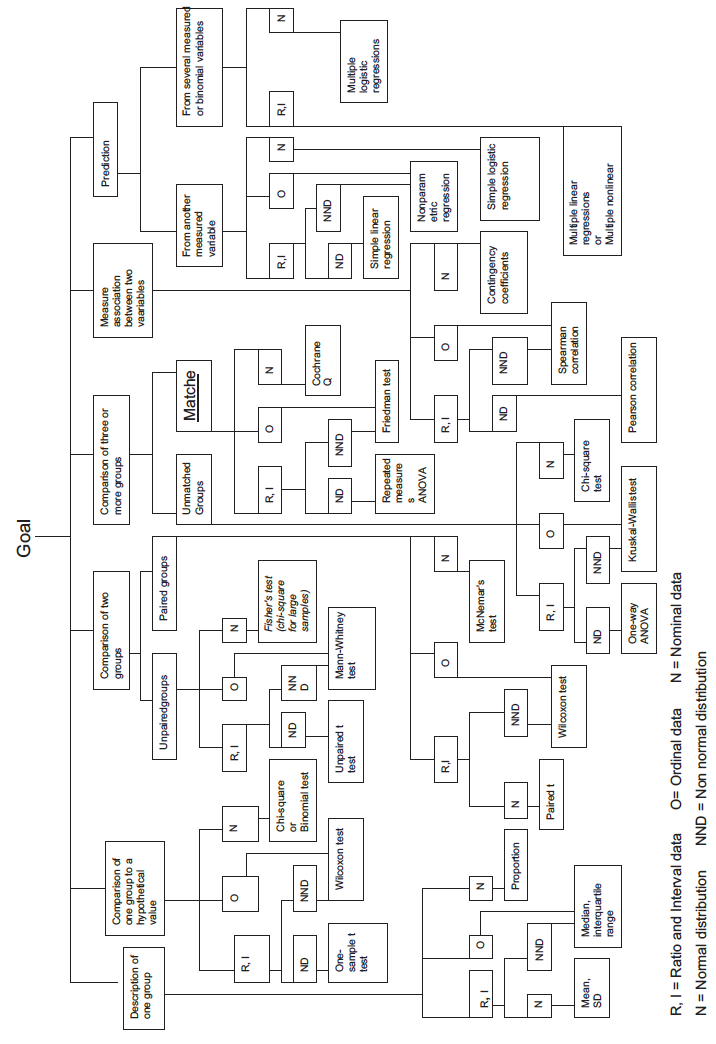
\includegraphics[width=.9\linewidth]{Flowchart.png}  
  \caption{Flowchart for the selection of appropriate statistical tests}
  \label{fig1}
\end{figure}


\textbf{i) What are the assumptions to apply parametric techniques?}\\

There are four important assumptions when it comes to the use of parametric tests in the analysis of data \cite{verma2019}, which are listed in Listing \ref{list2}.

\begin{itemize}\label{list2}
\item \textbf{Normal distribution data:} The \texttt{p}-value depends on a normal sampling distribution. If the sample size is big enough and the sample data point value are aproximately normally distributed, then the central limit ensures a normally distributed distribution.
\item \textbf{Homogeneity of variance:} The variable in the population where we took the samples have been taken in similar variance of these populations.
\item \textbf{Interval data:} The data point values should be for numerical variable and measured at this level.
\item \textbf{Independence:} Data point values for variables for different groups should be independent of each other. In regression analysis, the errors should likewise be independent.
\end{itemize}

\section{Experimentation}

Using the same topic as practice 1, \say{Enviromental practices} from the page of INEGI \cite{inegi} we attempt to replicate as many statistical test as possible. In this case, we still use the tables from the water section, but because the behavior of the previous data was to fractured and not compatible with any of the tests, we are focusing now on the quality of certain services on urban spaces. In this case, they give a 100 percent, and distributed in bad, regular and good quality. \\

In R we made a variable with each distribution, hoping to get a more normally distributed data than the one that we used before. In Figure \ref{extra} we see the distribution of each variable. \\

\begin{figure}[]
\begin{subfigure}{.3\textwidth}
  \centering
  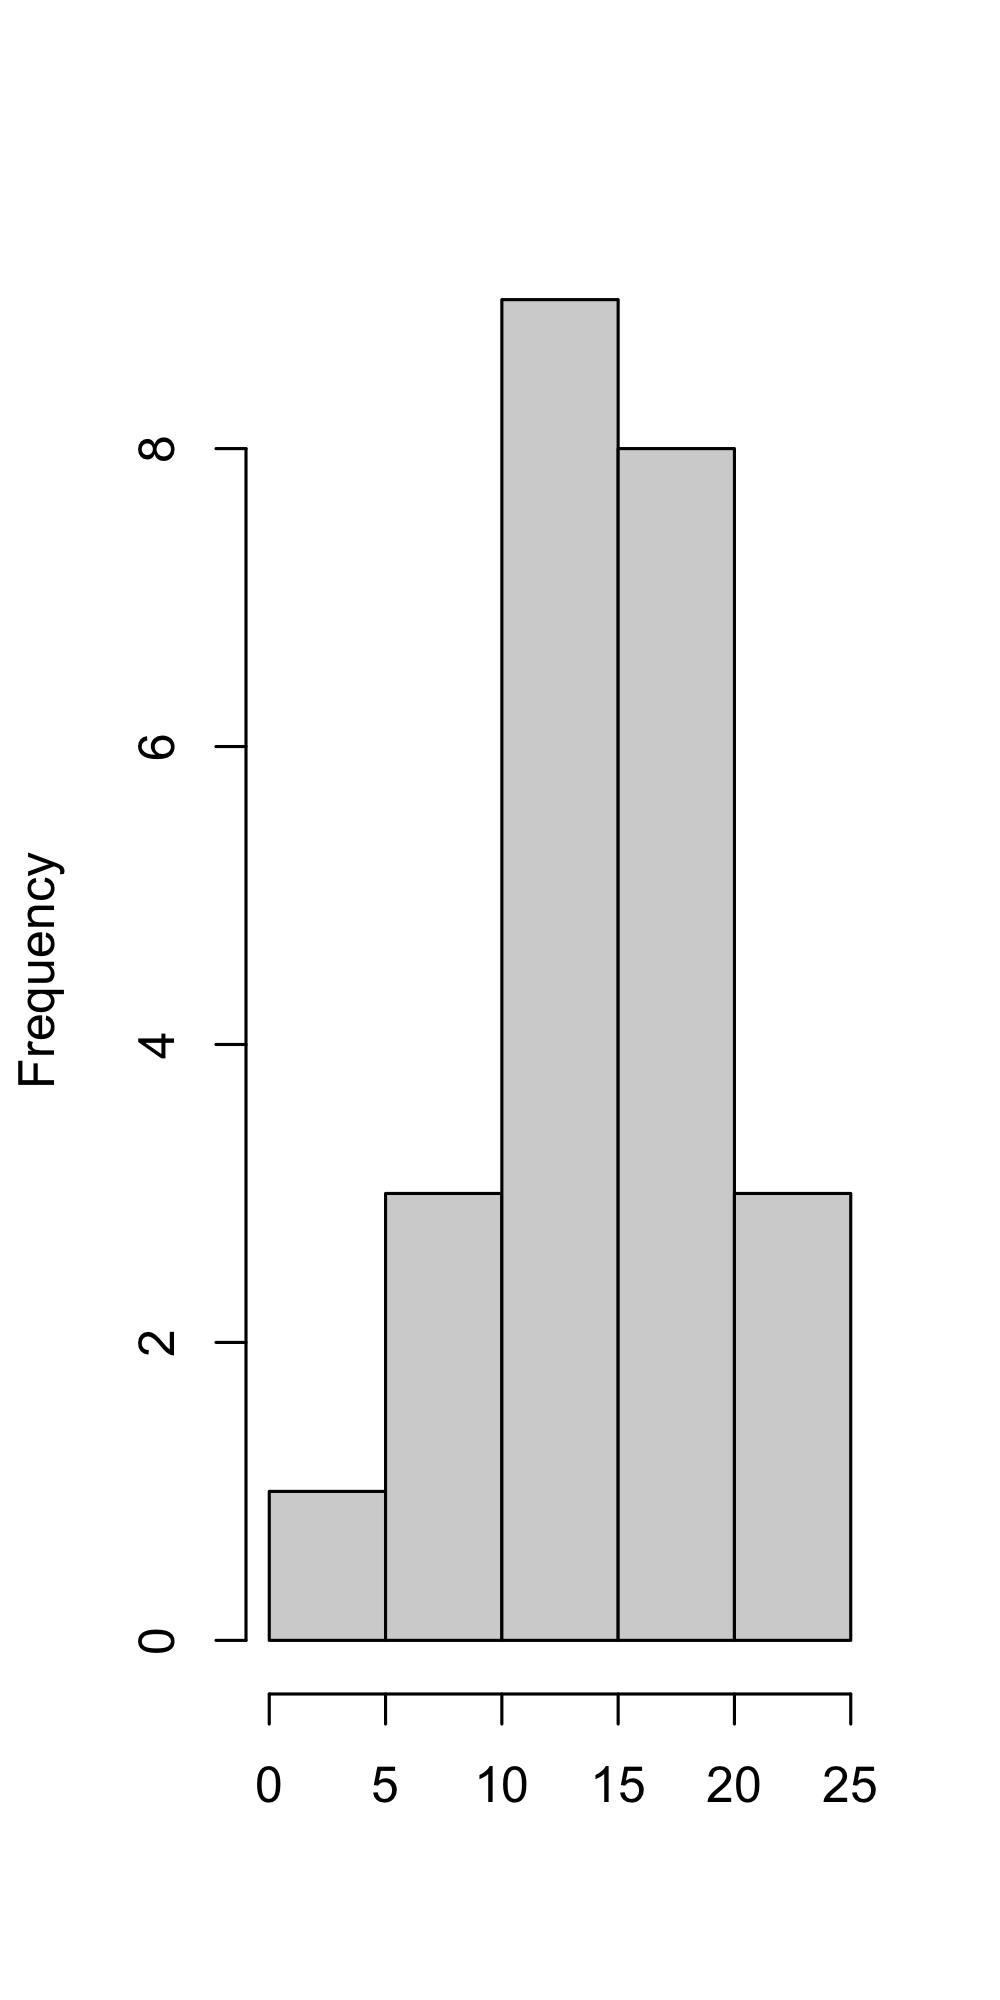
\includegraphics[width=.9\linewidth]{Ej6_malo.png}  
  \caption{Distribution of bad reviews }
  \label{extra1}
\end{subfigure}
\begin{subfigure}{.3\textwidth}
  \centering
  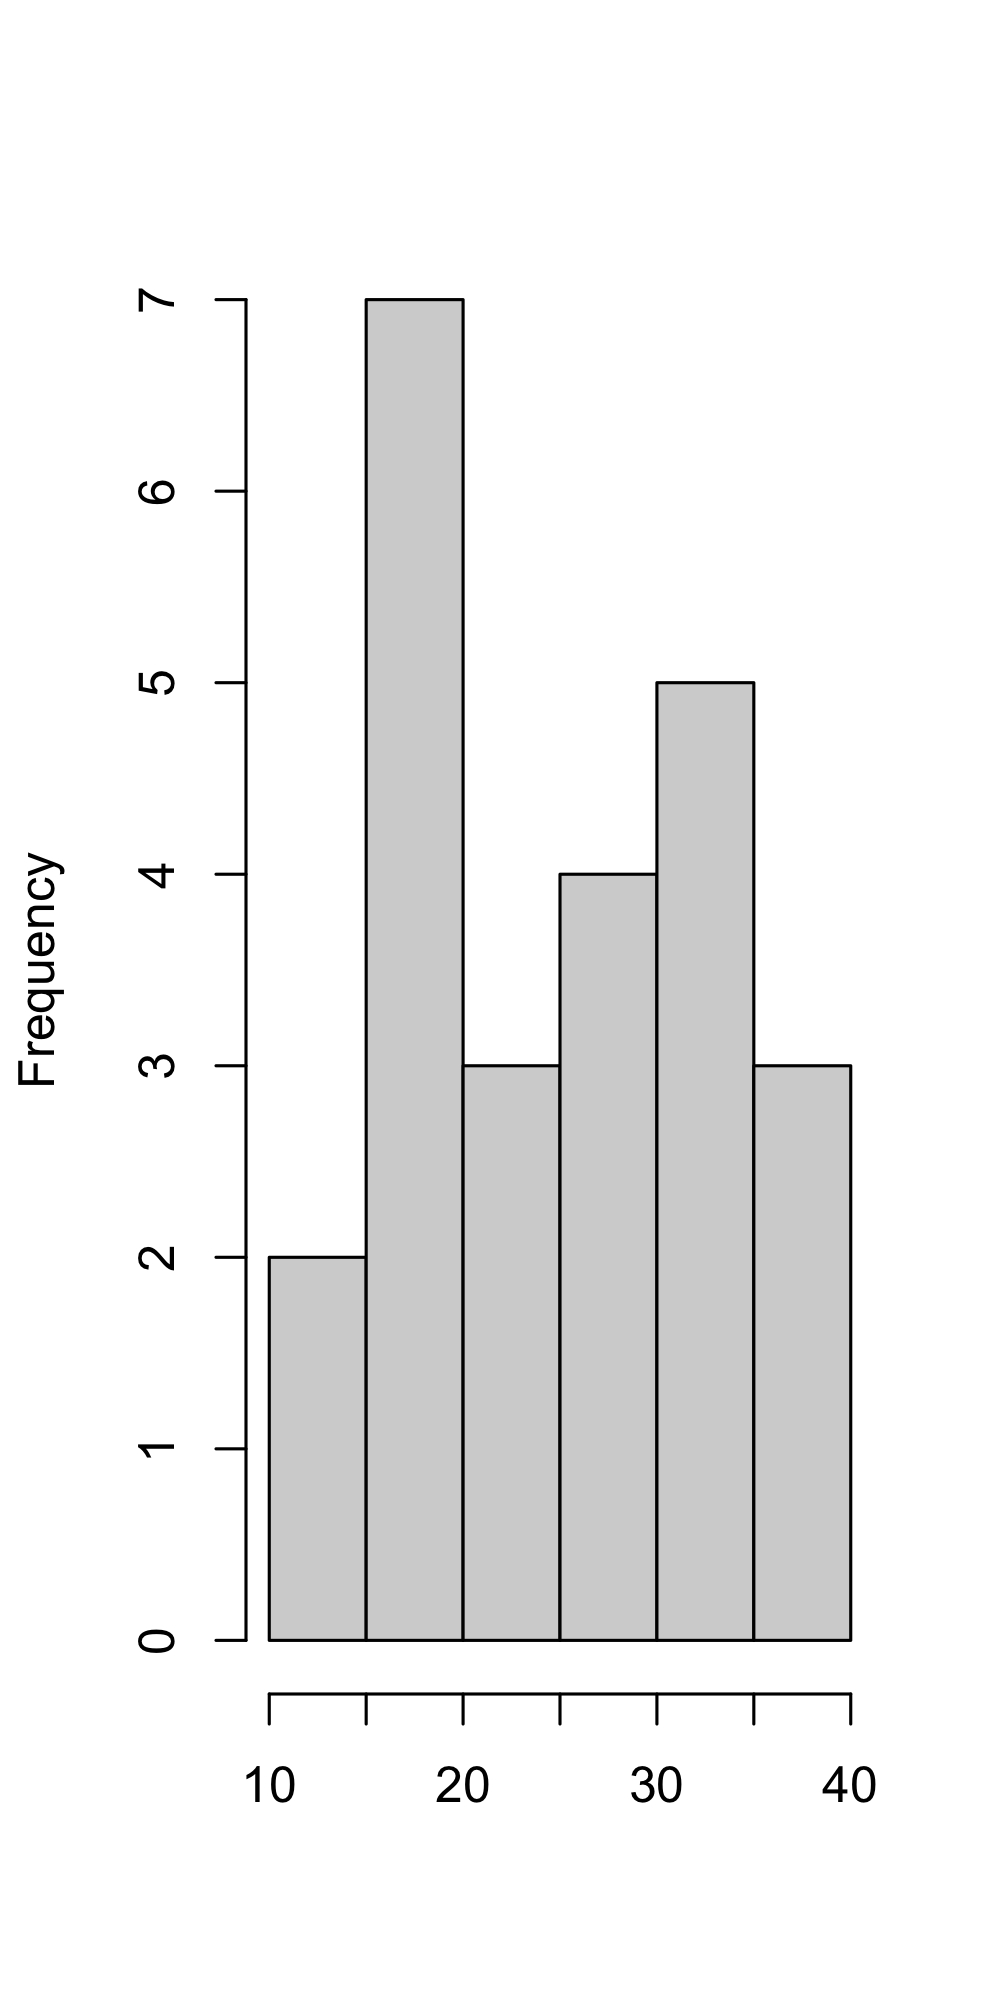
\includegraphics[width=.9\linewidth]{Ej6_regular.png}  
  \caption{Distribution of regular reviews}
  \label{extra2}
\end{subfigure}
\begin{subfigure}{.3\textwidth}
  \centering
  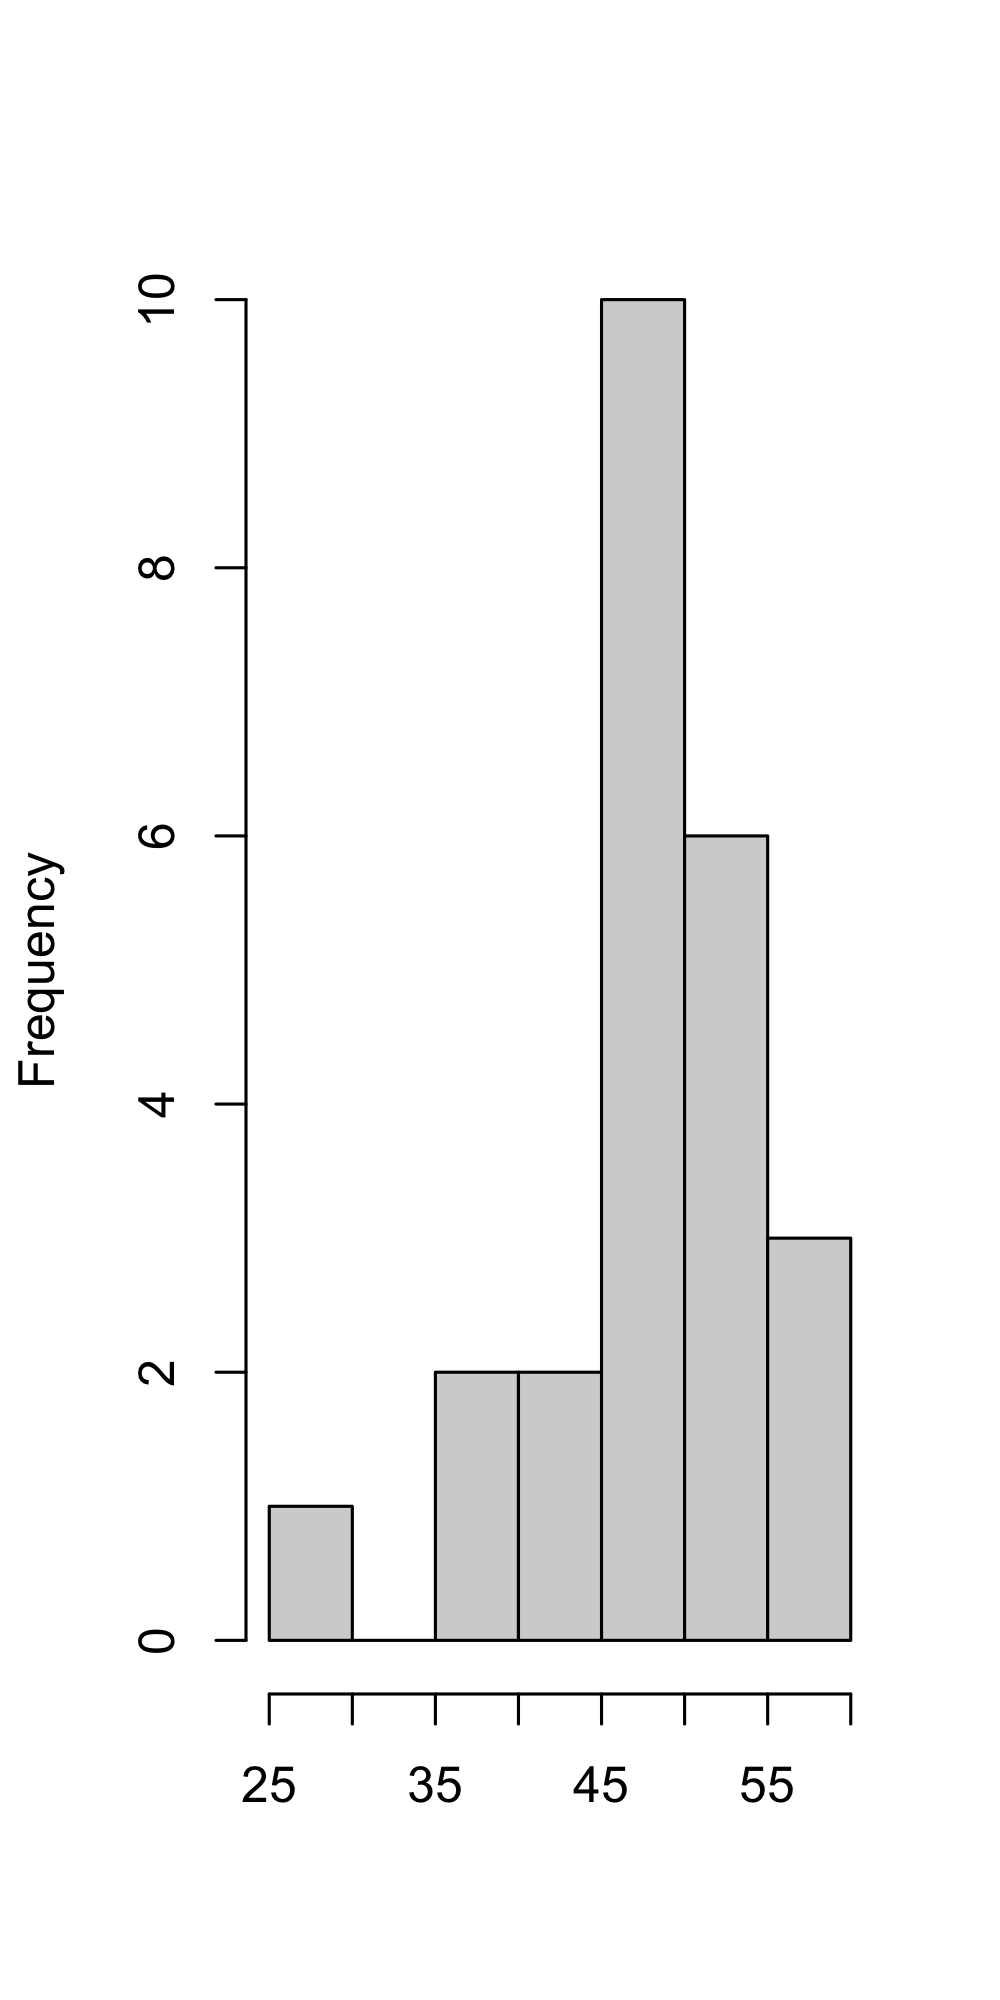
\includegraphics[width=.9\linewidth]{Ej6_bueno.png}  
  \caption{Distribution of good reviews}
  \label{extra3}
\end{subfigure}
\caption{Distribution of the public opinion about the water service of urban spaces.}
\label{extra}
\end{figure}

At plain sight we can speculate that Figure \ref{extra1} and \ref{extra2} are more or less resembling a normal distribution. But to be certain, we can perform some experimentation on the data. \\

\subsection{One sample t-test}

This is a parametric test to prove if the mean of a sample from a normal distribution could reasonably be a specific value. This test needs as values the name of the data, and a number that represents the posible mean. Seeing all three histograms, we set this parameter in each one as 15, 25, and 45, because is the most central in each one. \\

The results of the test are shown in Table \ref{tab3}.\\

\begin{table}[]\caption{Output in R of the One sample t-test.}\label{tab3}
\centering
\begin{tabular}{| l | c | c | c | c | c |}
\hline
&\multicolumn{5}{ c |}{One sample t-test variables}\\
\hline
Data& t & df & \texttt{p}-value & 95\% confidence  interval &Mean\\
\hline
Bad & -0.4531&  23& 0.6547 & 12.4916   --- 16.6067  & 14.54\\
\hline 
Regular & 0.0600 & 23 &  0.9527 & 21.8560   --- 28.3318 &25.09\\
\hline 
Good &1.7898 & 23 &  0.0866 & 44.6074   ---   50.4312 & 47.51\\
\hline                                                 
\end{tabular}
\end{table}

Interpreting this results, we put our null hypothesis in each case that the mean of each data variable was 15, 25, and 45 for \texttt{bad},  \texttt{regular} and  \texttt{good} respectively. Seeing the results on Table \ref{tab3} we can see that in all three cases we accept the null hypothesis. In column mean we also can see that our first assumption to use the medium value of the histogram as mean was not so far off. The farthest one was the  \texttt{good} variable, and it was off only by 2.51.\\
 
\subsection{Wilcoxon Signed Rank Test}

We move to a experimentation to test the mean of a sample when normal distribution is not assumed of the data. In Table \ref{tab4} we see the results of this test on each variable.\\

\begin{table}[]\caption{Output in R of the Wilcoxon signed rank test.}\label{tab4}
\centering
\begin{tabular}{| l | c | c | c | c |}
\hline
&\multicolumn{4}{ c |}{Wilcoxon variables}\\
\hline
Data& V & \texttt{p}-value &   95\% confidence  interval &Pseudo median\\
\hline
Bad & 141&  0.8115&  12.4177 --- 16.8965  & 14.77\\
\hline 
Regular & 151 & 0.9888 &   21.6393 --- 28.4672&25.15\\
\hline 
Good & 234& 0.0150 &   45.7382 --- 50.6462 & 48.25\\
\hline                                                 
\end{tabular}
\end{table}

In this case, without the assumption of normality in our distribution the \texttt{p}-value, we reject the null hypothesis on the \texttt{good} variable. The difference in the media is also a bit larger in all three variables.\\

\subsection{Shapiro test}

This test is used to see if our sample follows a normal distribution. Same as the experiments before, we are going to check if all of our variables follow a normal distribution. Table \ref{tab5} shows the results of this test.\\


\begin{table}[]\caption{Output in R of the Shapiro test.}\label{tab5}
\centering
\begin{tabular}{| l | c | c | }
\hline
&\multicolumn{2}{ c |}{Shapiro test variables}\\
\hline
Data& W & \texttt{p}-value \\
\hline
Bad & 0.9664&  0.5814\\
\hline 
Regular & 0.9485 &0.2515 \\
\hline 
Good & 0.8776& 0.0074 \\
\hline                                                 
\end{tabular}
\end{table}

As expected, variables \texttt{bad} and \texttt{regular} pass the test as normal distribution, but the \texttt{good} variable does not. \\

\subsection{Kolmogorov and Smirnov test}

This test helps find out if two samples follow the same distribution. From Figure \ref{extra} we can see that the distribution of our variables are different, but in Table \ref{tab6} we prove it further than just analyzing a figure.\\


\begin{table}[]\caption{Output in R of the Kolmogorov-Smirnov test.}\label{tab6}
\centering
\begin{tabular}{| l | c | c | }
\hline
&\multicolumn{2}{ c |}{Kolmogorov-Smirnov variables}\\
\hline
Data& D & \texttt{p}-value \\
\hline
Bad and Good & 1.0000&  6.195$\times10^{-14}$\\
\hline 
Regular and Good & 0.9166 &6.996$\times10^{-11}$ \\
\hline 
Bad and Regular &0.6250& 0.0001 \\
\hline                                                 
\end{tabular}
\end{table}

\subsection{Fisher F-test}

This test can be used to check if two samples have the same variance. We used the same parings as the Kolmogorov-Smirnov test. The results can be seen in Table \ref{tab7}. In this case, all three variables pass the null hypothesis, and the ratio of variances gives us also a positive result between them.\\

\begin{table}[]\caption{Output in R of the Fisher F-test.}\label{tab7}
\centering
\begin{tabular}{| p{1.5cm}  | c | c | c | c | c | p{1.4cm} |}
\hline
&\multicolumn{6}{ c |}{Fisher F-test variables}\\
\hline
Data& F & num df &   denom df &\texttt{p}-value & 95\% confidence interval & Ratio of variances\\
\hline
Bad and Good & 0.4993&  23&  123  & 0.1028&0.2159 --- 1.1541&0.4992 \\
\hline 
Regular and Good&  1.2364&  23&  23  & 0.6150&0.5348 --- 2.8582&1.2364\\
\hline 
Bad and Regular & 0.4038& 23 &   23& 0.0343 & 0.1746 --- 0.9334 & 0.4038\\
\hline                                                 
\end{tabular}
\end{table}


\subsection{Correlation}

This test gives us as a result the linear relationship of the two continuous variables. The null hypothesis in this case is that the true correlation between both variables is zero. The results of this tests are shown in Table \ref{tab8}.\\

\begin{table}[]\caption{Output in R of the correlation test.}\label{tab8}
\centering
\begin{tabular}{| p{1.5cm}  | c | c | c | c | c |}
\hline
&\multicolumn{5}{ c |}{Correlation variables}\\
\hline
Data& t & df &  \texttt{p}-value & 95\% confidence interval & Correlation\\
\hline
Bad and Good & 1.5459&  22&  0.1364&-0.1034 ---  0.6360&0.3130 \\
\hline 
Regular and Good&  2.7261&  22  & 0.0123& 0.1242 --- 0.7532&0.5024 \\
\hline 
Bad and Regular & 2.9768& 22 & 0.0069 &0.1689 --- 0.7723 & 0.5358 \\
\hline                                                 
\end{tabular}
\end{table}

In this case the null hypothesis of the correlation could only be accomplished by the pair of \texttt{bad} and \texttt{good} variables.

\section{Other experimentation}

We have talked and experimented with different known statistical tests. And even if now when, after all the research they seem a lot more understandable, visual queues remain a favorite. So, after some searching, we found other ways to show our data. In Figure \ref{fig9} we have the Q-Q plot, or more commonly known as the quantile-quantile plot. It helps to assess if a set of data came from some distribution such as normal or exponential.\\

This is the visual check of something that the t-test does, which is assume that the variable is normally distributed, so it is not a complete proof, but something to help visualize the data. In the case of Figure \ref{fig9} we compare our results with Table \ref{tab3}, and we find similar results.\\

\begin{figure}[]
\begin{subfigure}{.3\textwidth}
  \centering
  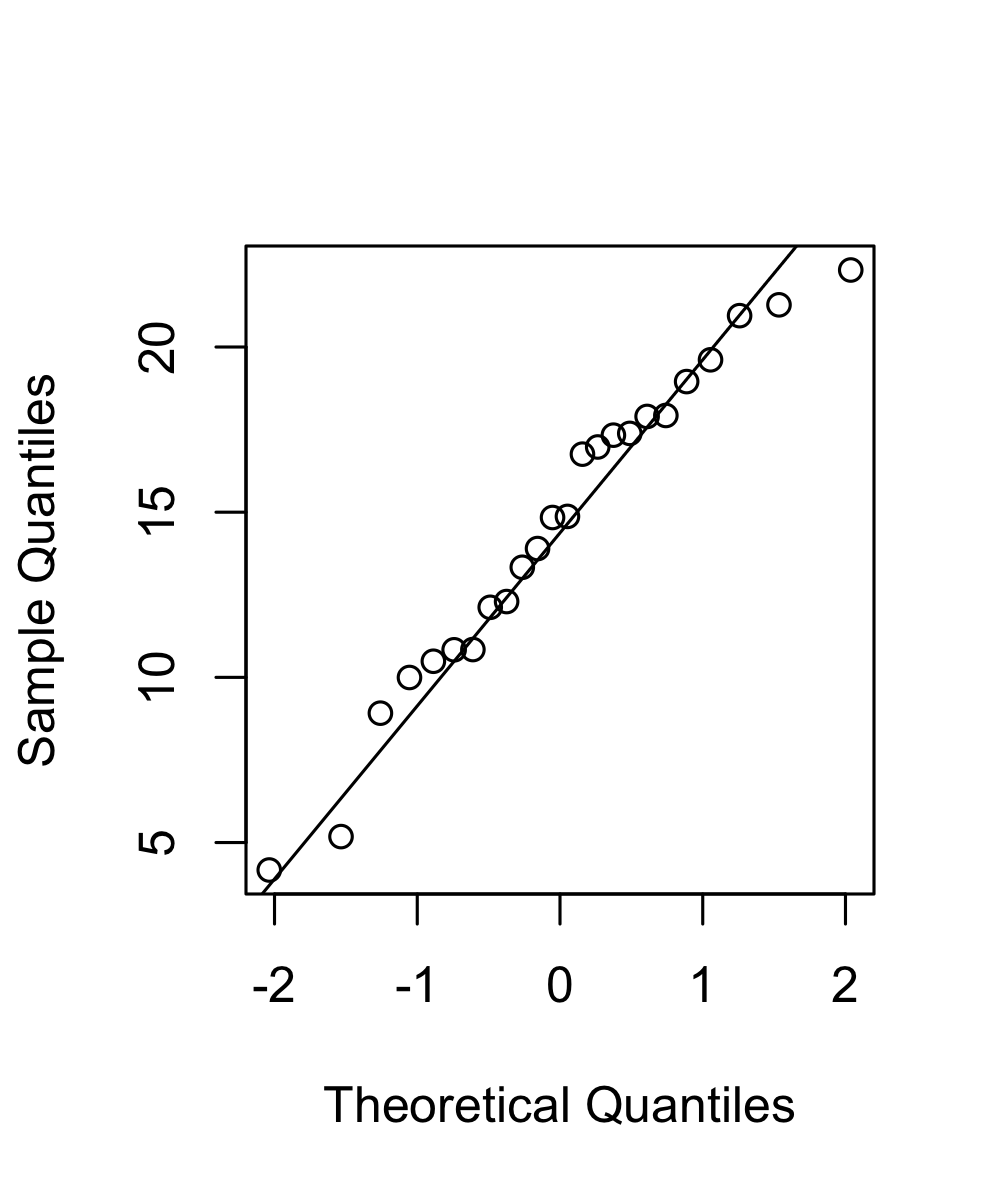
\includegraphics[width=1\linewidth]{Ej6_maloqq.png}  
  \caption{Normal Q-Q plot of bad reviews }
  \label{sf1}
\end{subfigure}
\begin{subfigure}{.3\textwidth}
  \centering
  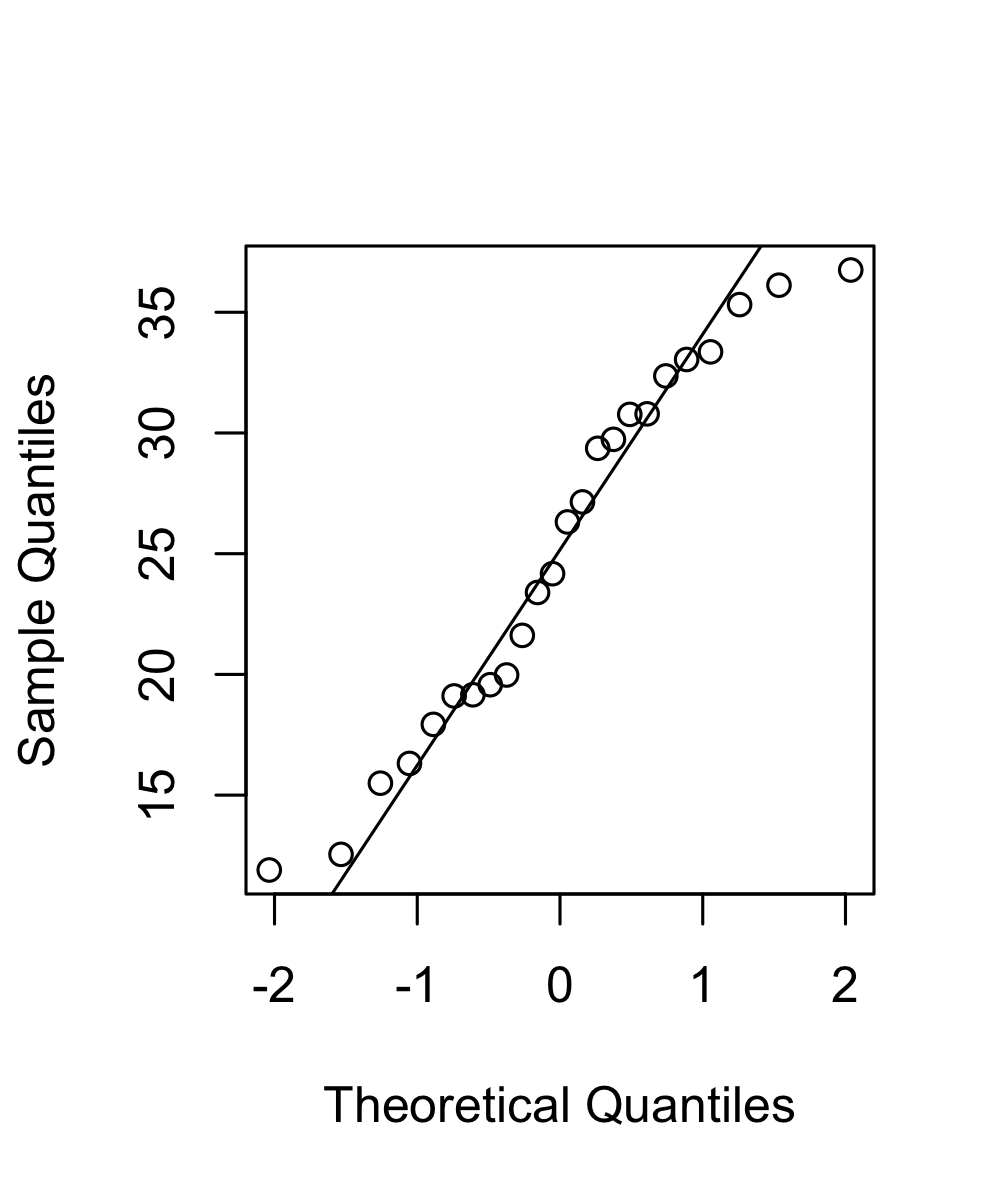
\includegraphics[width=1\linewidth]{Ej6_regularqq.png}  
  \caption{Normal Q-Q plot of regular reviews}
  \label{sf2}
\end{subfigure}
\begin{subfigure}{.3\textwidth}
  \centering
  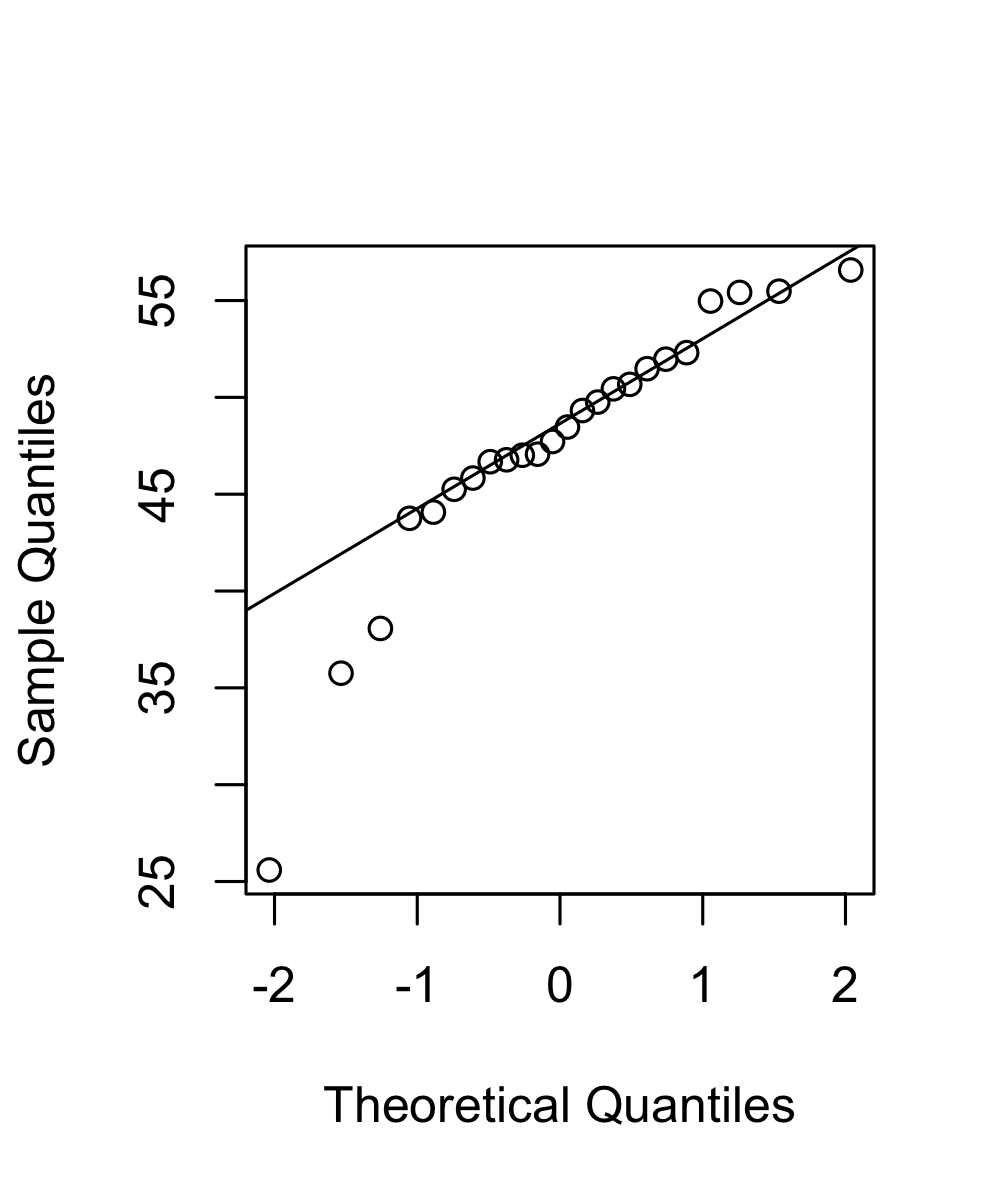
\includegraphics[width=1\linewidth]{Ej6_buenoqq.png}  
  \caption{Normal Q-Q plot of good reviews}
  \label{sf3}
\end{subfigure}
\caption{Normal Q-Q plot of all the variables}
\label{fig9}
\end{figure}


Another visual queue besides the histograms if Figure \ref{extra} to help find the mean of our data are the box plots. In Figure \ref{fig99} we show the box plots of all the variables. Here we can see more clearly the mean of each variable, as well as the odd behavior of some of the data in variable \texttt{Good}.\\

\begin{figure}[]
\begin{subfigure}{.3\textwidth}
  \centering
  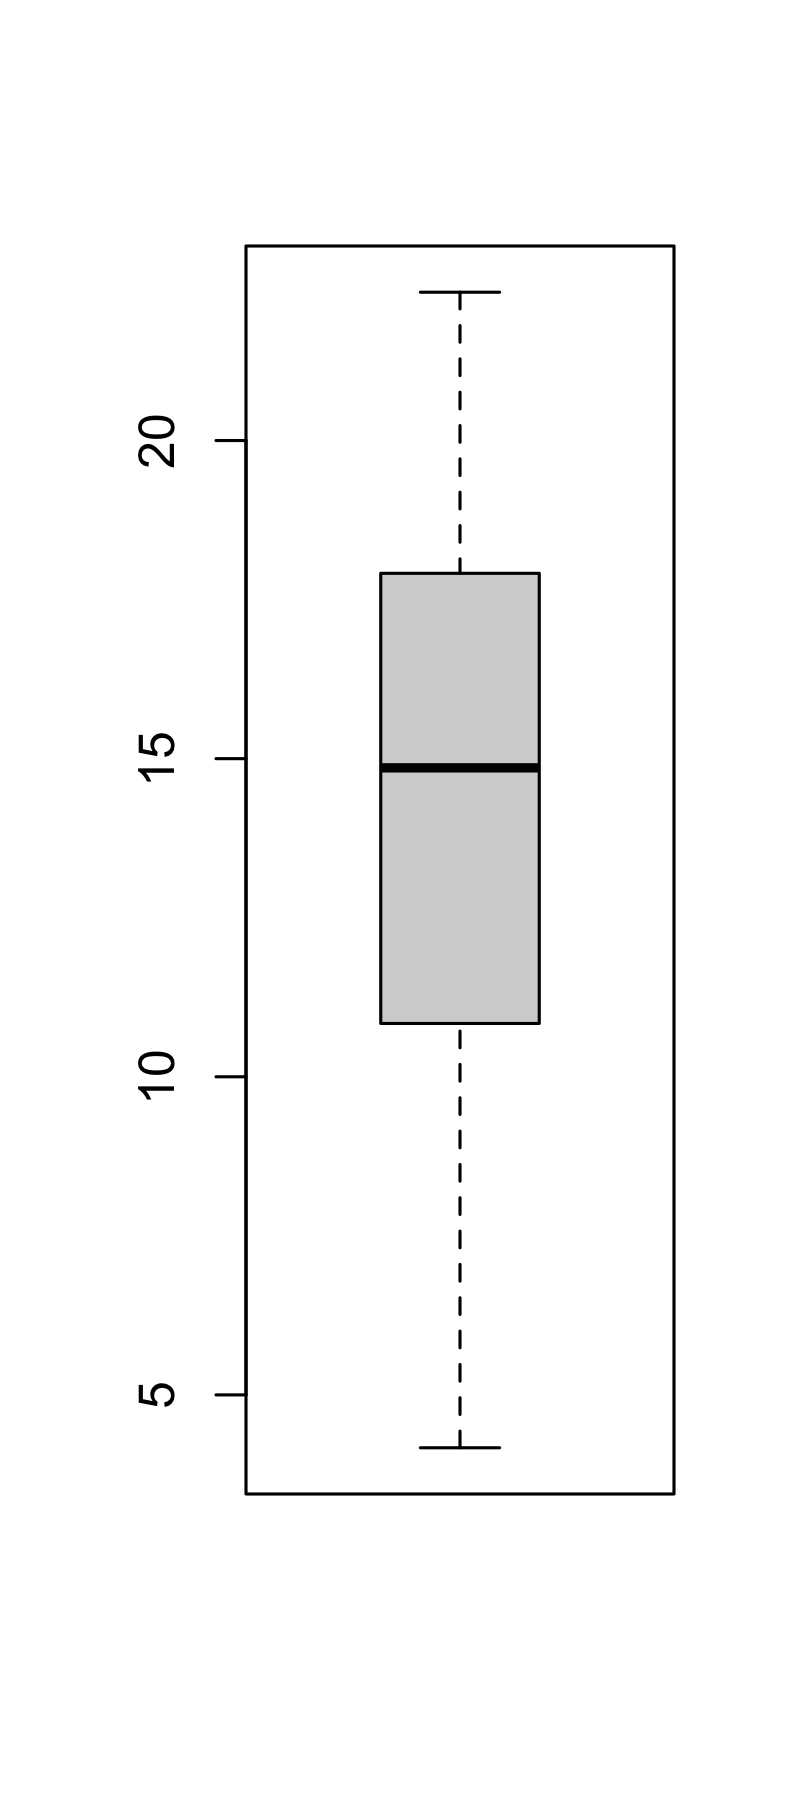
\includegraphics[width=.9\linewidth]{Ej6_malobox.png}  
  \caption{Box plot of bad reviews }
  \label{sf91}
\end{subfigure}
\begin{subfigure}{.3\textwidth}
  \centering
  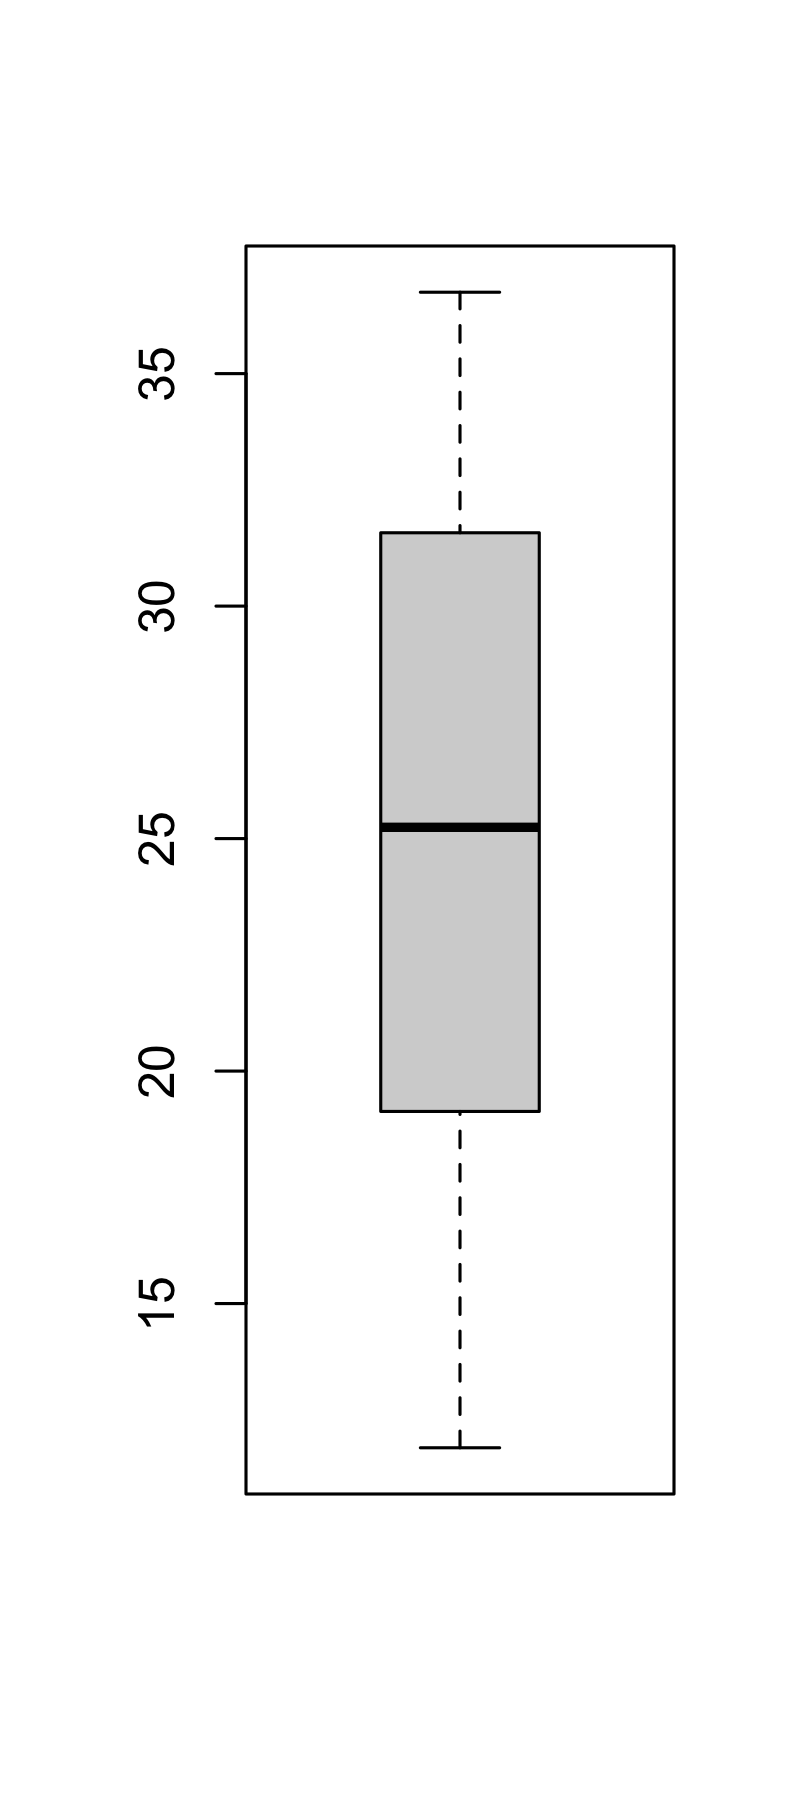
\includegraphics[width=.9\linewidth]{Ej6_regularbox.png}  
  \caption{Box plot of regular reviews}
  \label{sf92}
\end{subfigure}
\begin{subfigure}{.3\textwidth}
  \centering
  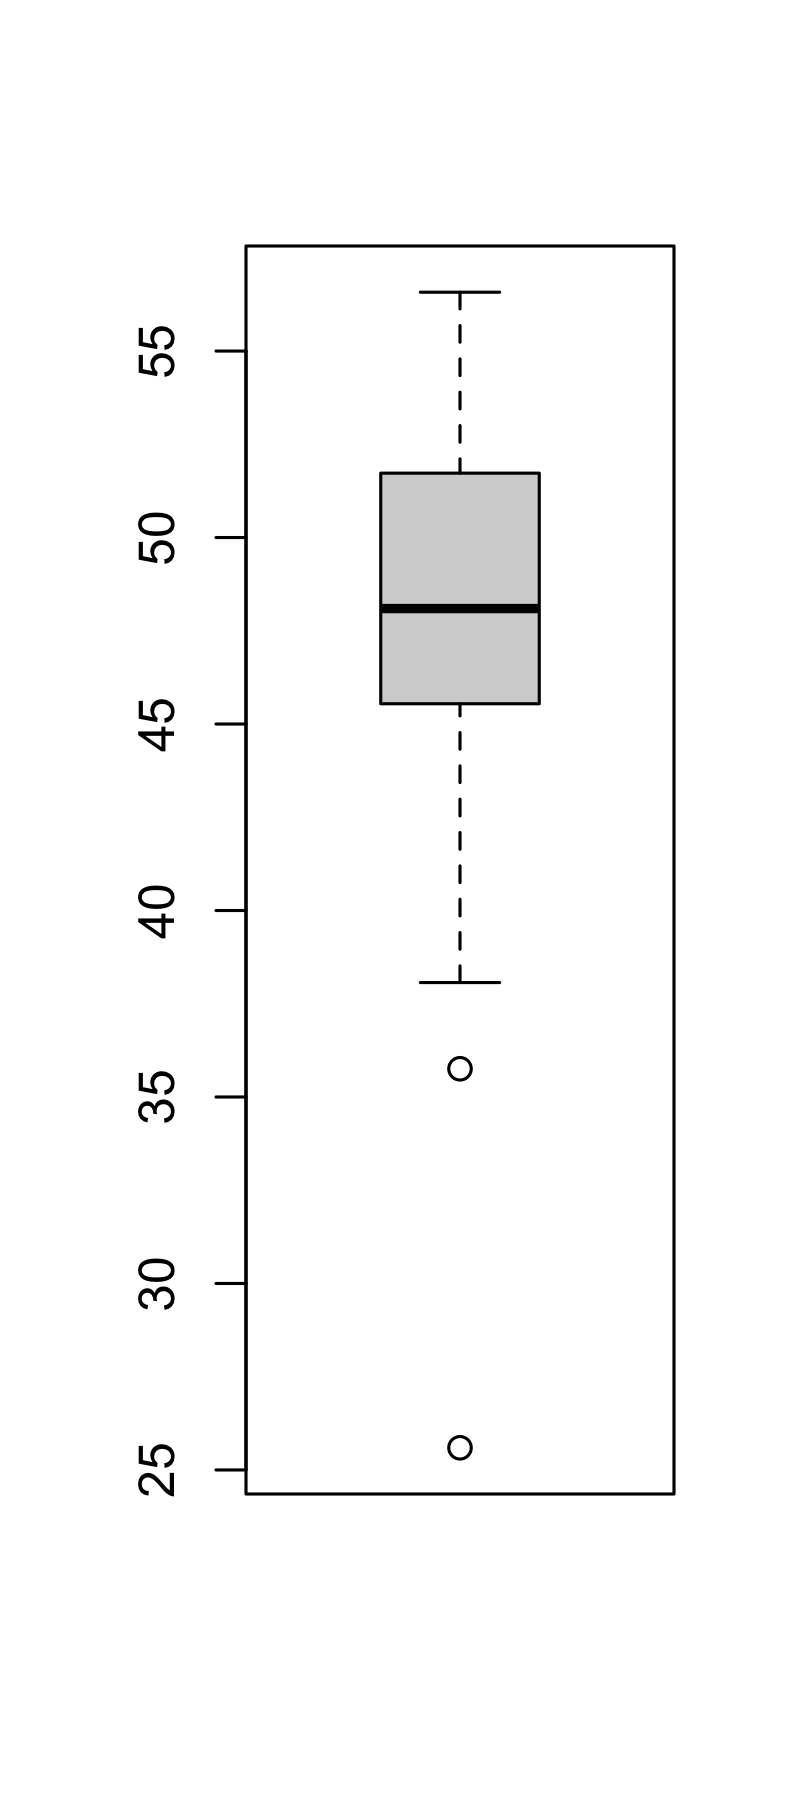
\includegraphics[width=.9\linewidth]{Ej6_buenobox.png}  
  \caption{Box plot of good reviews}
  \label{sf93}
\end{subfigure}
\caption{Box plots of all the variables}
\label{fig99}
\end{figure}

\section{Conclusions}

So far I was understanding fine the histograms and plots made in class, but in the last practice one of the mayor faults in my work was that I misinterpreted some data. With this practice the concepts of the tests and their results are clearer. They can help us move from just guessing our answers from the plots and actually proving some points, because many of the articles and books researched for this practice say that plots are only visual aids, and should require a bit more experimentation to back them up.\\

\bibliographystyle{plainnat}
\bibliography{tarea6}


 
\end{document}